%%
%% This is file `sample-manuscript.tex',
%% generated with the docstrip utility.
%%
%% The original source files were:
%%
%% samples.dtx  (with options: `manuscript')
%% 
%% IMPORTANT NOTICE:
%% 
%% For the copyright see the source file.
%% 
%% Any modified versions of this file must be renamed
%% with new filenames distinct from sample-manuscript.tex.
%% 
%% For distribution of the original source see the terms
%% for copying and modification in the file samples.dtx.
%% 
%% This generated file may be distributed as long as the
%% original source files, as listed above, are part of the
%% same distribution. (The sources need not necessarily be
%% in the same archive or directory.)
%%
%% The first command in your LaTeX source must be the \documentclass command.
%%%% Small single column format, used for CIE, CSUR, DTRAP, JACM, JDIQ, JEA, JERIC, JETC, PACMCGIT, TAAS, TACCESS, TACO, TALG, TALLIP (formerly TALIP), TCPS, TDSCI, TEAC, TECS, TELO, THRI, TIIS, TIOT, TISSEC, TIST, TKDD, TMIS, TOCE, TOCHI, TOCL, TOCS, TOCT, TODAES, TODS, TOIS, TOIT, TOMACS, TOMM (formerly TOMCCAP), TOMPECS, TOMS, TOPC, TOPLAS, TOPS, TOS, TOSEM, TOSN, TQC, TRETS, TSAS, TSC, TSLP, TWEB.
% \documentclass[acmsmall]{acmart}

%%%% Large single column format, used for IMWUT, JOCCH, PACMPL, POMACS, TAP, PACMHCI
% \documentclass[acmlarge,screen]{acmart}

%%%% Large double column format, used for TOG
% \documentclass[acmtog, authorversion]{acmart}

%%%% Generic manuscript mode, required for submission
%%%% and peer review
\documentclass[manuscript,screen]{acmart}

%%
%% \BibTeX command to typeset BibTeX logo in the docs
\AtBeginDocument{%
  \providecommand\BibTeX{{%
    \normalfont B\kern-0.5em{\scshape i\kern-0.25em b}\kern-0.8em\TeX}}}

%% Rights management information.  This information is sent to you
%% when you complete the rights form.  These commands have SAMPLE
%% values in them; it is your responsibility as an author to replace
%% the commands and values with those provided to you when you
%% complete the rights form.
%\setcopyright{acmcopyright}
\copyrightyear{2020}
%\acmYear{2020}
%\acmDOI{10.1145/1122445.1122456}

%% These commands are for a PROCEEDINGS abstract or paper.
%\acmConference[Woodstock '18]{Woodstock '18: ACM Symposium on Neural
 % Gaze Detection}{June 03--05, 2018}{Woodstock, NY}
%\acmBooktitle{Woodstock '18: ACM Symposium on Neural Gaze Detection,
 % June 03--05, 2018, Woodstock, NY}
%\acmPrice{15.00}
%\acmISBN{978-1-4503-XXXX-X/18/06}

%%
%% end of the preamble, start of the body of the document source.
\begin{document}

%%
%% The "title" command has an optional parameter,
%% allowing the author to define a "short title" to be used in page headers.
\title{Revisiting AR Piano}

%%
%% The "author" command and its associated commands are used to define
%% the authors and their affiliations.
%% Of note is the shared affiliation of the first two authors, and the
%% "authornote" and "authornotemark" commands
%% used to denote shared contribution to the research.
\author{Jordan Aiko Deja}
%\authornote{Both authors contributed equally to this research.}
\email{jordan.deja@famnit.upr.si}
\orcid{1234-5678-9012}
\affiliation{%
  \institution{University of Primorska}
  \city{Koper}
  \country{Slovenia}
  \postcode{6000}
}

%\author{Matjaž Kljun and Klen Čopič Pucihar}
%\affiliation{%
%  \institution{Advisors}
%  \city{Koper}
 % \postcode{6000}}
%\email{\{matjaz.kljun, klen.copic\}@famnit.upr.si}

%\author{Klen Čopič Pucihar}
%\affiliation{%
%  \institution{University of Primorska}
 % \city{Koper}
  %\country{Slovenia}
  %\postcode{6000}}
%\email{klen.copic@famnit.upr.si}

%%
%% By default, the full list of authors will be used in the page
%% headers. Often, this list is too long, and will overlap
%% other information printed in the page headers. This command allows
%% the author to define a more concise list
%% of authors' names for this purpose.
\renewcommand{\shortauthors}{Deja, et al.}
%%
%% The abstract is a short summary of the work to be presented in the
%% article.
\begin{abstract}
\textbf{Abstract:} Humans have been using and learning the piano for over 3 centuries. In the last 15 years, several Augmented Reality (AR) piano prototypes that support learning have been introduced. Why are we still building these prototypes? What do these systems lack? In this paper, we present a systematic review of AR piano prototypes developed within the recent years. We review the different innovations they present and organise them into contribution categories. We will then discuss the impact of these contributions and recommend directions for future work towards designing better AR piano prototypes. 
\end{abstract}
%%
%% The code below is generated by the tool at http://dl.acm.org/ccs.cfm.
%% Please copy and paste the code instead of the example below.
%%
\begin{CCSXML}
<ccs2012>
   <concept>
       <concept_id>10003120.10003121.10003126</concept_id>
       <concept_desc>Human-centered computing~HCI theory, concepts and models</concept_desc>
       <concept_significance>500</concept_significance>
       </concept>
   <concept>
       <concept_id>10003120.10003145</concept_id>
       <concept_desc>Human-centered computing~Visualization</concept_desc>
       <concept_significance>100</concept_significance>
       </concept>
 </ccs2012>
\end{CCSXML}
\ccsdesc[500]{Human-centered computing~HCI theory, concepts and models}
\ccsdesc[100]{Human-centered computing~Visualization}
%%
%% Keywords. The author(s) should pick words that accurately describe
%% the work being presented. Separate the keywords with commas.
\keywords{extended reality, spatiotemporal pointing, piano, music teaching ystems}
%%
%% This command processes the author and affiliation and title
%% information and builds the first part of the formatted document.
\maketitle

\section{Introduction}
Survey of AR piano teaching systems and prototypes
Discussion on how these prototypes were evaluated and how the research focus has changed over the last 15 years
Overview of what technological contributions were made and future steps 

.. This paper focuses on X prototypes categorized and sorted by .. These sections describe prototypes that addressed problems in (enumerate). In each section, prototypes are grouped in subsection compared by its .. They are also listed in chronological order to show the course of development. Each subsection ends with a short discussion about .. This paper concludes with an overview discussion and a conclusion about ..

\section{Background}
Augmented Reality
Augmented reality piano teaching systems
Design Factors affecting augmented reality piano teaching systems (hardware, software, content)

\section{Method}
Meta-analysis (Search for prototypes, Inclusion criteria, data gathering)
Qualitative Analysis (search for prototype, inclusion criteria, data gathering)
How did you do the review? What were the sources and keywords used? What was the qualifying criteria? 
How did you organize the prototypes? By what categories? How is the rest of the document then sorted based on these categories? 

\section{Trends in AR Piano Prototypes}
\section{Strategies in Designing AR Pianos}
\subsection{Visualisations}
Section discussing prototypes whose main contributions focused on visualizations, overlaying graphics, rendering and optimization etc
\subsection{Agents and Tutors}
Section discussing prototype whose main contributions focused on virtual agents/tutors 
\subsection{Learning Modes}
Section discussing prototype whose contributions focused on learning modes, emphasis on pedagogy and other learner-centric modes
\section{Evaluation Techniques}
done by studies on AR piano teaching systems (hypothesis based on cognition, realistic annotations etc)
\section{Discussion and Future Directions}
\section{Tables and Figures}
Figure of number of participants per study by years, size of each bubble is relative to sizes of other bubbles and based on number of participants in a study. Sort per category 

Figure/Table of all described prototypes with year, by type with number of participants, short study description, number of citations

Table of Studies evaluating learner performance with effect sizes (content, sample, control group, treatment, effect, size)

Table of Studies evaluating learner performance 

Figure of number of AR piano teaching system publications until june 2020

Table of AR piano teaching systems with corresponding devices 

Table of AR piano teaching systems showing summary of survey
questionnaires

\begin{figure}
    \centering
    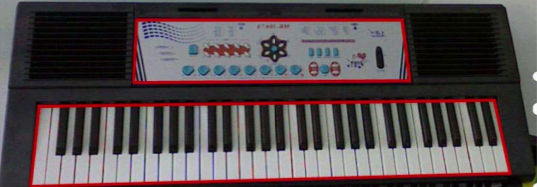
\includegraphics[width=15cm]{figures/pianomarker.png}
    \caption{Piano Augmented Reality marker}
    \label{fig:pianomarker}
\end{figure}

\begin{figure}
    \centering
    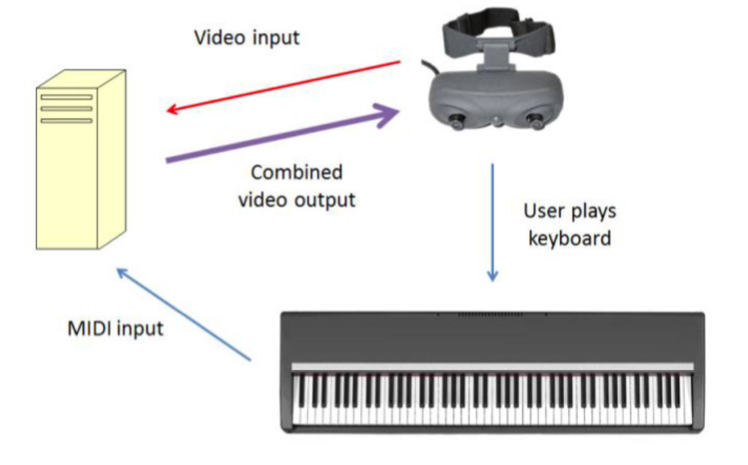
\includegraphics[width=10cm]{figures/headmountedpiano1.png}
    \caption{Architecture of the Head Mounted Piano by cite! }
    \label{fig:pianoheadmountedarch}
\end{figure}

\begin{figure}
    \centering
    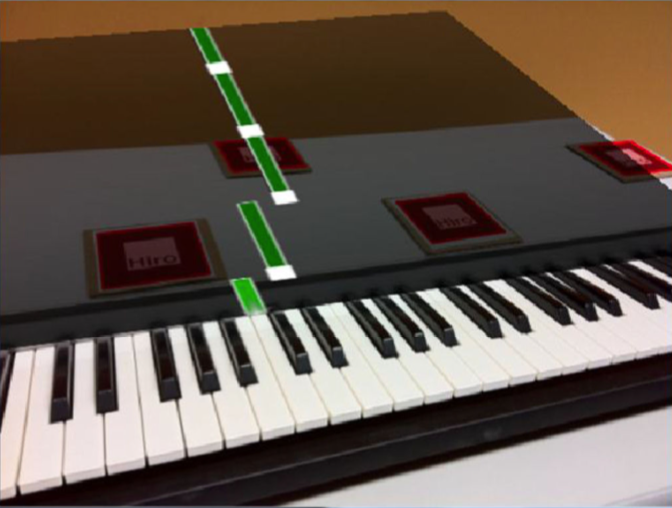
\includegraphics[width=10cm]{figures/headmountedview.png}
    \caption{View from the Head Mounted Piano AR  }
    \label{fig:View from the HeadMounted}
\end{figure}

\begin{figure}
    \centering
    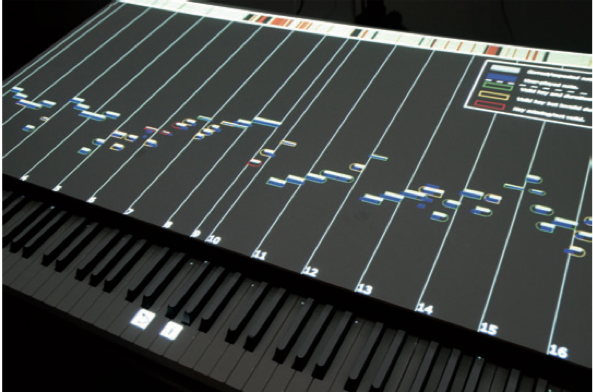
\includegraphics[width=10cm]{figures/piano}
    \caption{View of the Detailed Screen of P.I.A.N.O.› }
    \label{fig:View from the HeadMounted}
\end{figure}









%%
%% The next two lines define the bibliography style to be used, and
%% the bibliography file.
\bibliographystyle{ACM-Reference-Format}
\bibliography{sample-base}
%%
%% If your work has an appendix, this is the place to put it.
%\appendix
\end{document}
\endinput
%%
%% End of file `sample-manuscript.tex'.
